\documentclass[titlepage,landscape]{seminar}
\usepackage{url}
\usepackage{graphicx}
\usepackage[pdftex]{color}
\usepackage{hyperref}
\usepackage{epstopdf}
\usepackage{slides}

\begin{document}

\myslide{
\begin{table}
\begin{center}
\begin{tabular}{l|ccc}
\hline\hline
         & 5' flanking & {\it Adh\/} locus & 3' flanking \\
\hline
Diversity$^1$ \\
\quad Observed & 9     & {\bf 14}   & 2    \\
\quad Expected & 10.8  & 10.8 & 3.4  \\
Divergence$^2$ \\
\quad Observed & 86    & 48   & 31   \\
\quad Expected & 55    & {\bf 76.9} & 33.1 \\
\hline
\multicolumn{4}{l}{\footnotesize $^1$Number of polymorphic sites within {\it
         D. melanogaster\/}} \\
\multicolumn{4}{l}{\footnotesize $^2$Number of nucleotide differences between {\it
         D. melanogaster\/} and {\it D. simulans}}
\end{tabular}
\end{center}
\caption{Diversity and divergence in the {\it Adh\/} region of {\it
    Drosophila}~(from Kreitman and Aguade 1986).}
\end{table}
}

\myslide{
\begin{center}
\resizebox{0.8\textwidth}{!}{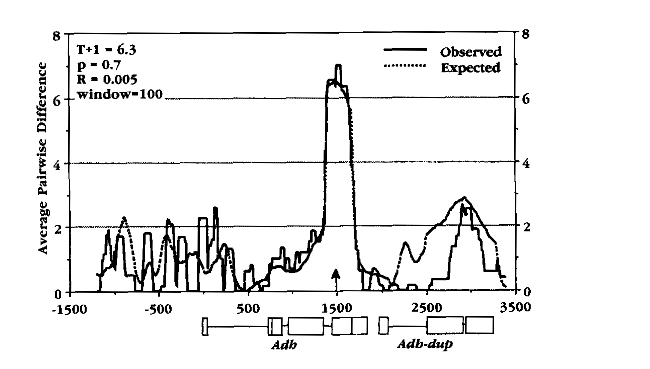
\includegraphics{kreitman-hudson.eps}}
\end{center}
}

\myslide{
\begin{center}
\resizebox{0.9\textwidth}{!}{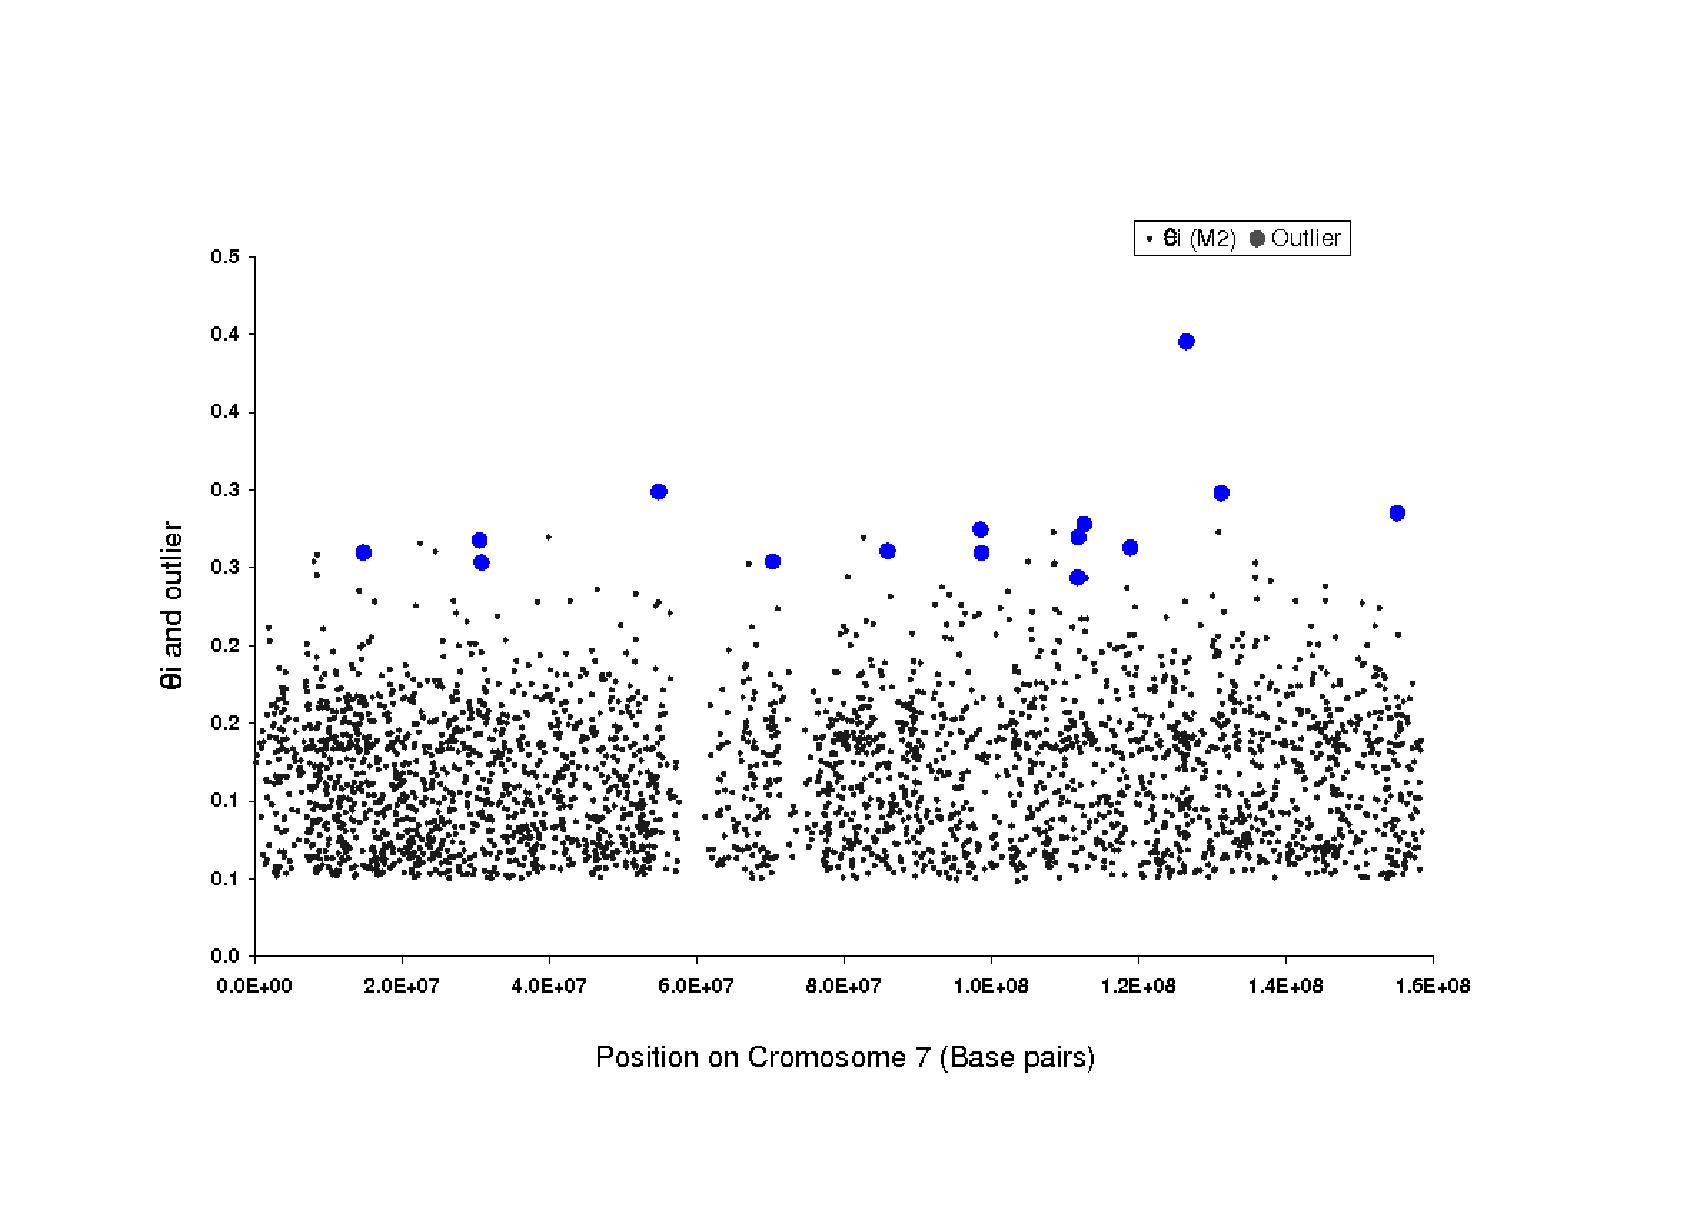
\includegraphics{outlier.eps}}
\end{center}
}

\myslide{
Average per nucleotide diversity
\begin{eqnarray*}
\pi &=& \sum x_ix_j\delta_{ij}/N \\
x_i &=& \mbox{frequency of haplotype $i$} \\
\delta_{ij} &=& \mbox{number of nucleotide differences between $i$ and
  $j$} \\
N &=& \mbox{length of haplotype sequence}
\end{eqnarray*}
}

\myslide{
Definition
\[
\theta = 4N_e\mu
\]
({\bf NOT} Weir \& Cockerham's $\theta$).
}

\myslide{
Under the infinite sites model of evolution
\begin{eqnarray*}
\E(\pi) &=& \theta \\
\E(k) &=& \theta\sum_i^{n-1} \frac{1}{i} \\
n &=& \mbox{number of haplotypes in the sample}
\end{eqnarray*}
\vfil
\begin{eqnarray*}
\hat \theta_\pi &=& \hat \pi \\
\hat \theta_k   &=& \frac{k}{\sum_i^{n-1}\frac{1}{i}} \\
\hat D &=& \hat\theta_\pi - \hat\theta_k 
\end{eqnarray*}
}

\myslide{
\begin{description}

\item[$\hat D = 0$:] We have no evidence for changes in population
  size or for any particular pattern of selection at the
  locus.

\item[$\hat D < 0$:] The population size may be increasing or we may
  have evidence for purifying selection at this locus.

\item[$\hat D > 0$:] The population may have suffered a recent
  bottleneck (or be decreaing) or we may have evidence for
  overdominant selection at this locus.

\end{description}
}

\myslide{
\begin{eqnarray*}
\pi_t &=& \sum_{ij} x_{i\cdot}x_{j\cdot} \delta_{ij} \\
\pi_s &=& \frac{1}{K}\sum_{k=1}^K\sum_{ij} x_{ik}x_{jk}\delta_{ij} \\
\Phi_{st} &=& \frac{\pi_t - \pi_s}{\pi_t}
\end{eqnarray*}
}

\myslide{
\begin{center}
\resizebox{!}{6cm}{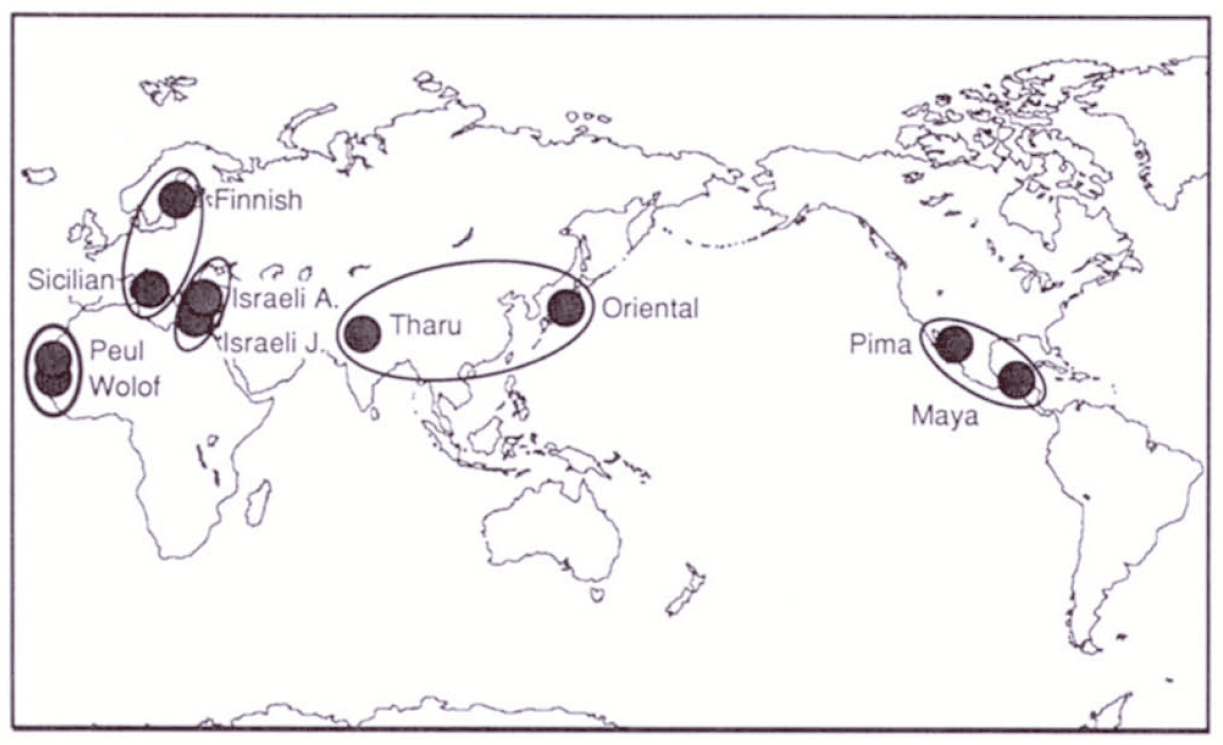
\includegraphics{amova-sample-locations.eps}}
\end{center}
}

\myslide{
\begin{center}
\resizebox{!}{6cm}{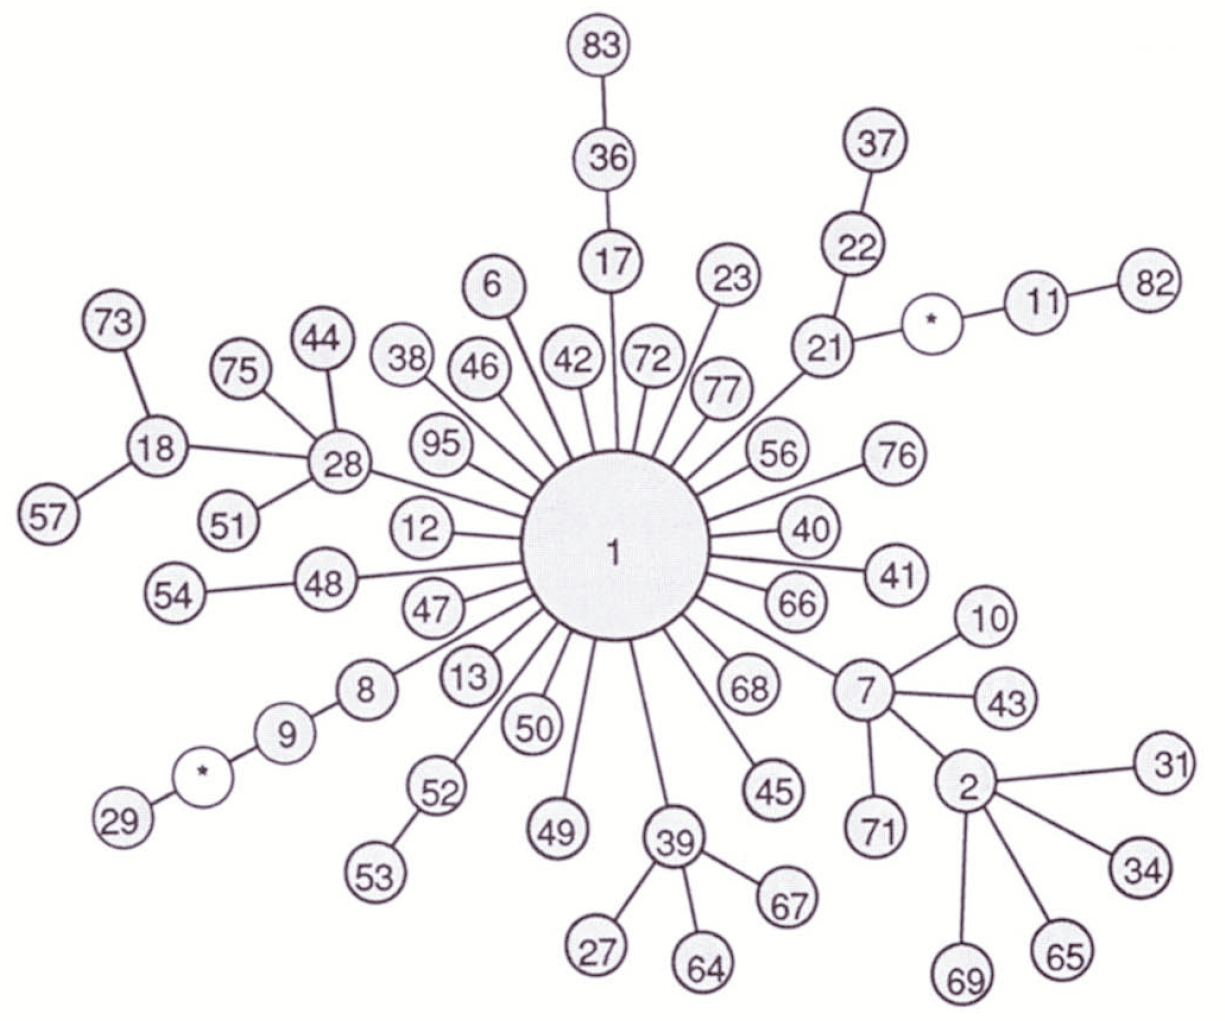
\includegraphics{amova-haplotypes.eps}}
\end{center}
}

\myslide{
\begin{center}
\begin{tabular}{lc}
\hline\hline
Component of differentiation     & $\Phi$-statistics \\
\hline
Among regions                    & $\Phi_{CT} = 0.220$ \\
Among populations within regions & $\Phi_{SC} = 0.044$ \\
Among all populations            & $\Phi_{ST} = 0.246$ \\
\hline
\end{tabular}
\end{center}
}

\myslide{
\begin{center}
\resizebox{!}{\textheight}{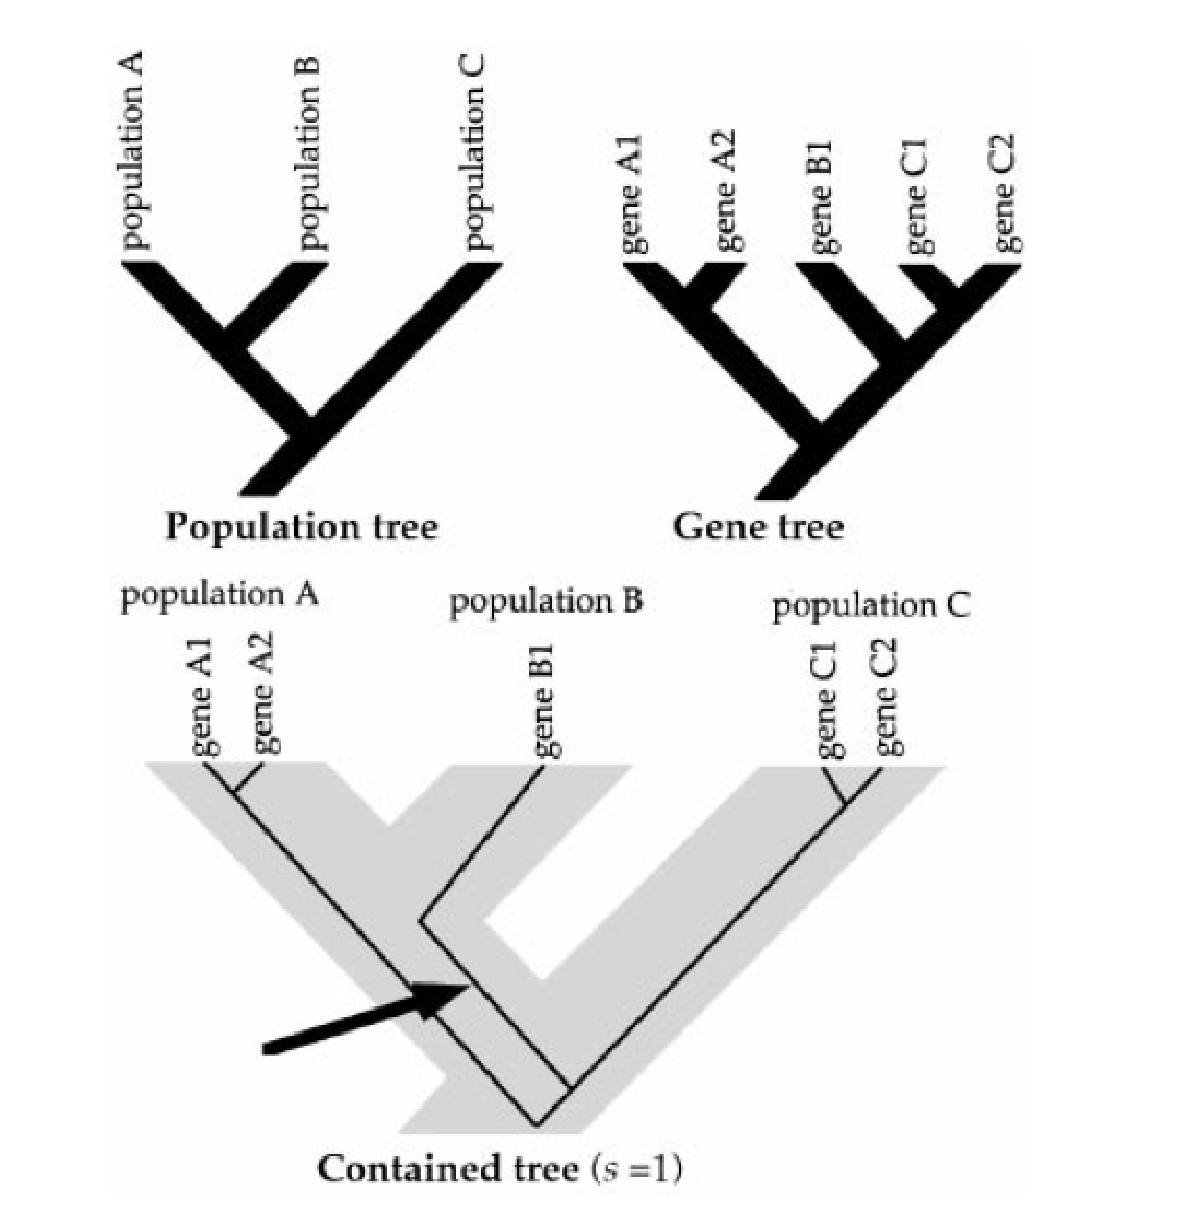
\includegraphics{ancestral-polymorphism.eps}}
\end{center}
}

\myslide{
\begin{center}
\resizebox{\textwidth}{!}{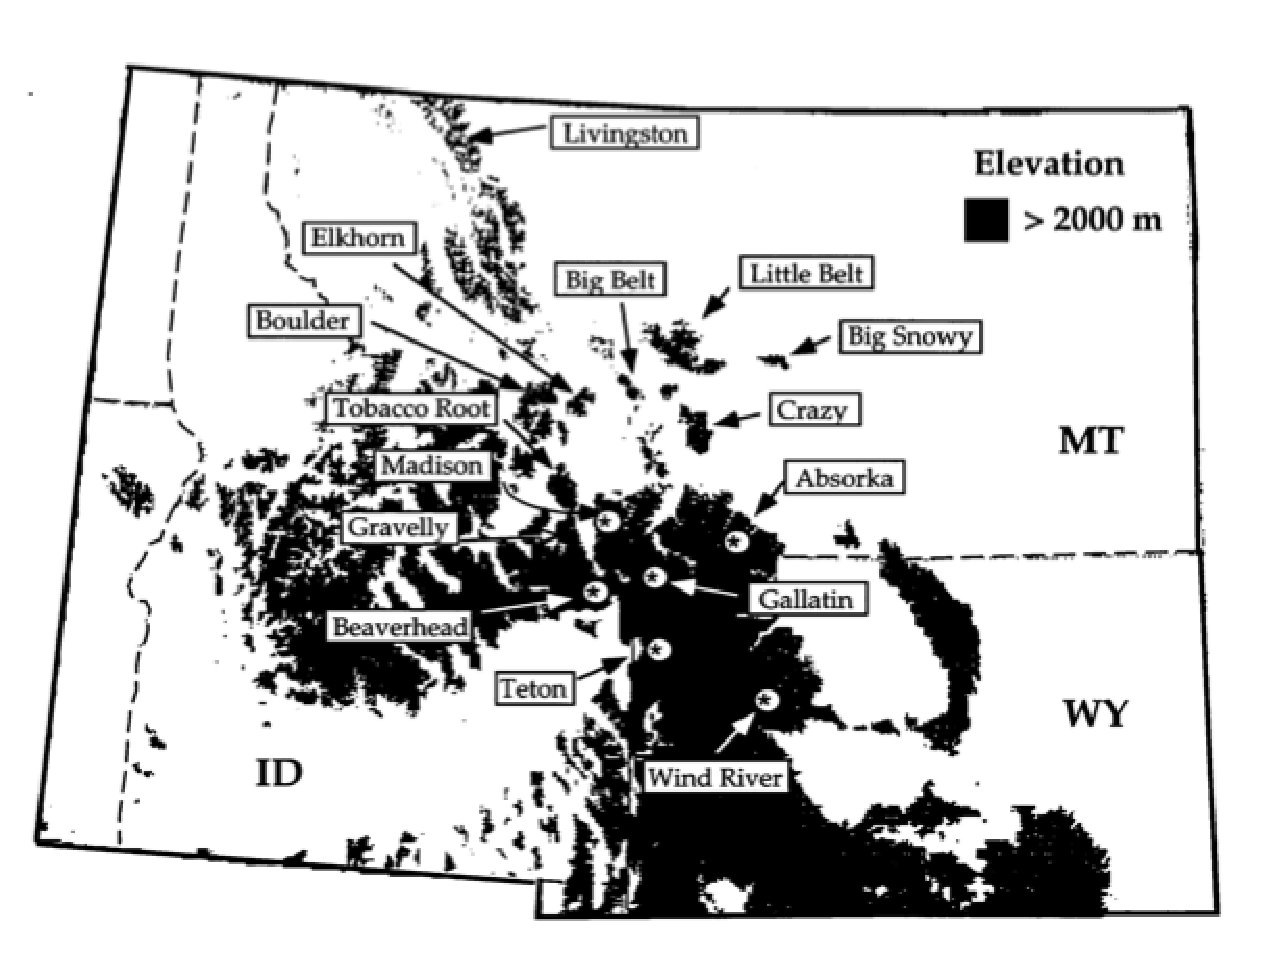
\includegraphics{sky-islands.eps}}
\end{center}
}

\myslide{
\begin{center}
\resizebox{!}{\textheight}{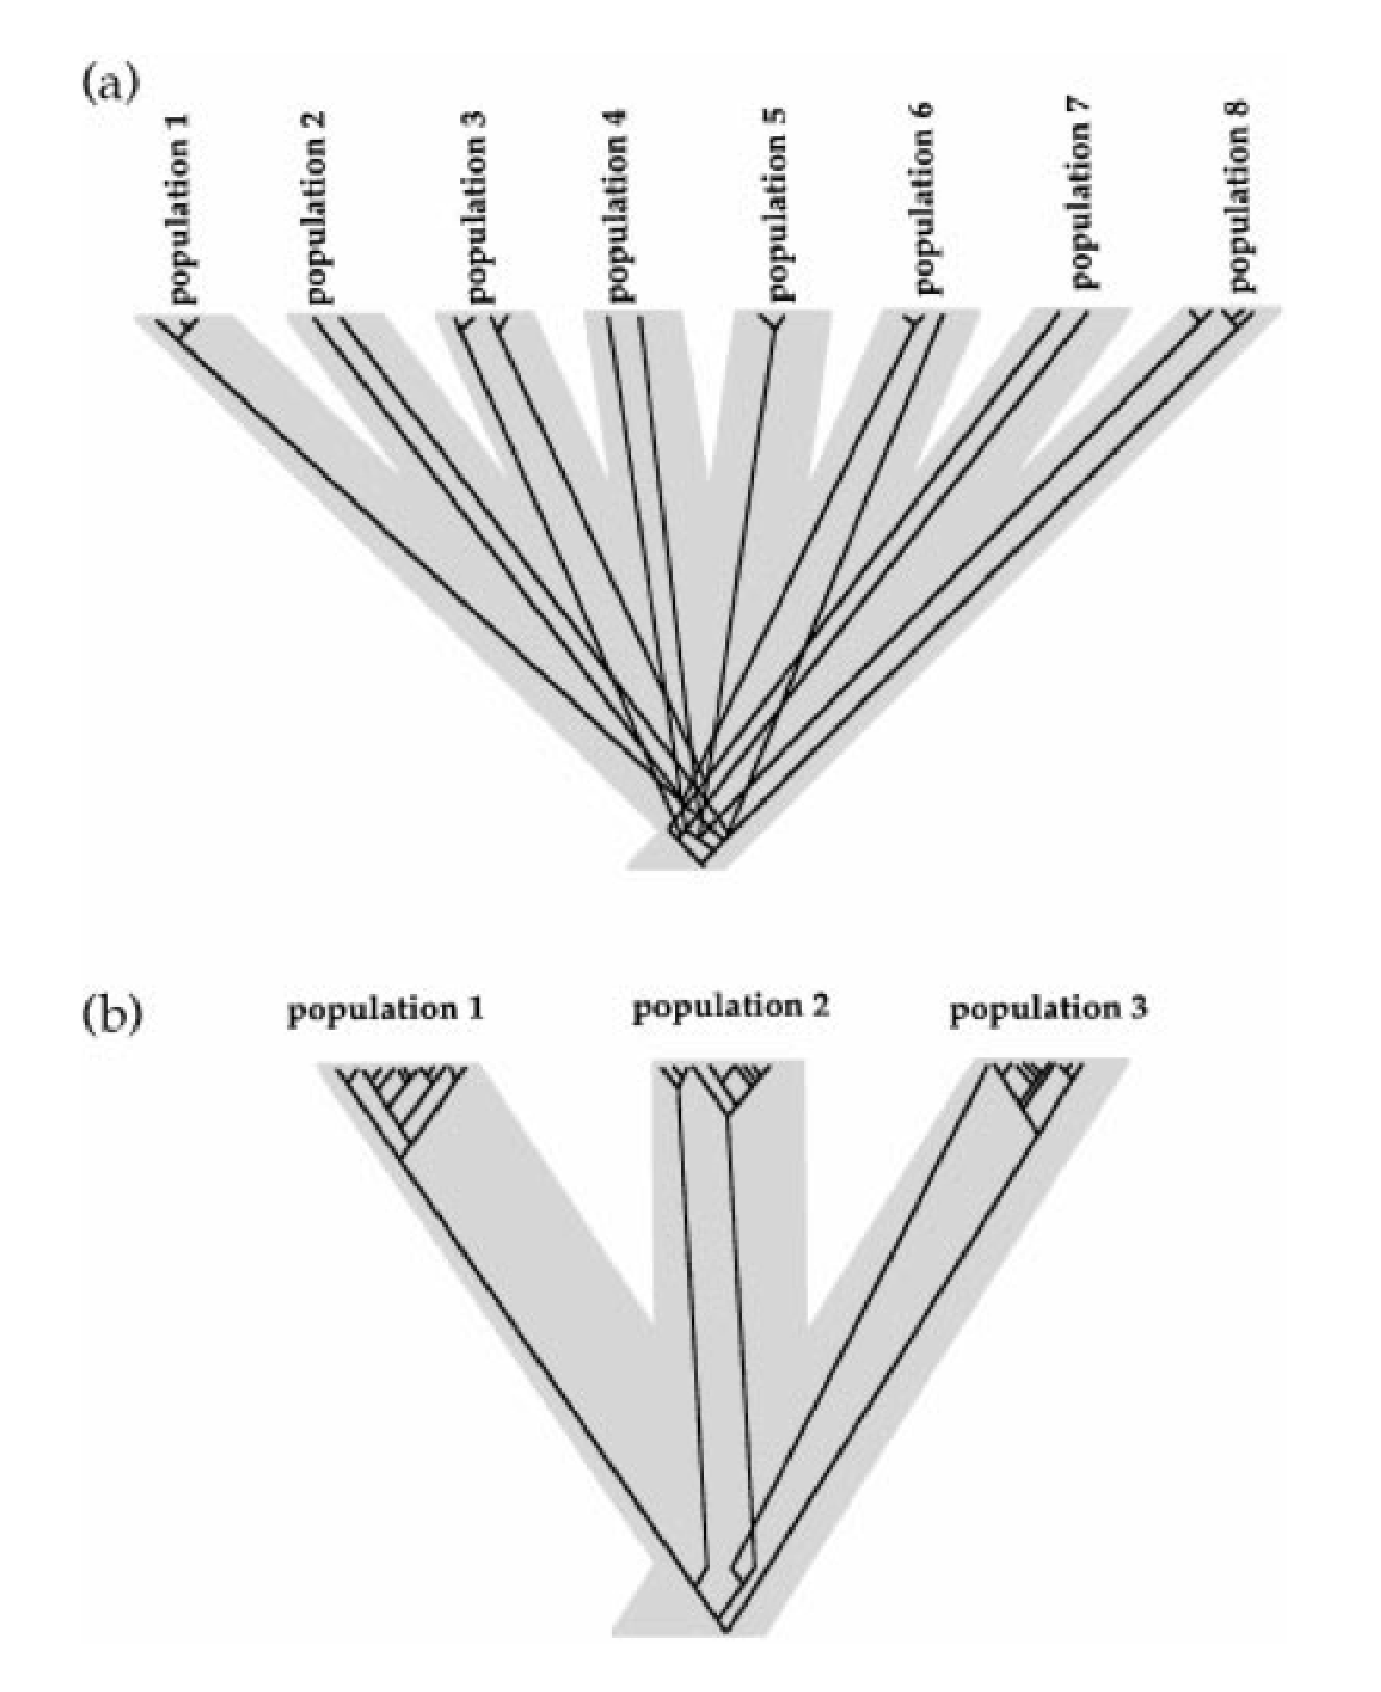
\includegraphics{divergence-hypotheses.eps}}
\end{center}
}

\end{document}

